\documentclass{scrbook}
\usepackage{indentfirst}
\usepackage{tikz}
\usepackage{amsmath}
\usepackage{pgfplots}
\usepackage{siunitx}
\usepackage{wrapfig}
\usepackage{circuitikz}
\usepackage[backend=bibtex]{biblatex}
\addbibresource{Physics.bib}
\title{Physics Notes}
\subtitle{A level Physics}
\date{Last Updated \today{}}
\author{Dhruva Lokegaonkar}
\begin{document}
\maketitle
\tableofcontents
\chapter{Circular Motion, Gravitation and Oscillation}

\section{Circular Motion}

\subsection{Measurement}
	Angles or angular displacement is usually measured in radians. $360^\circ = 2\pi rad$

	\begin{quote}
		One Radian is the angle subtended at the center of a circle by an arc of length equal to the radius of the circle
	\end{quote}

	The time period of rotation is $T$ and frequency is $f$

	\[ \omega = \frac{2\pi}{T} = 2\pi f \]

\subsection{Angular Velocity and Centripetal Force}

	The speed at which a object rotates is called it's angular velocity. It is measured in $rad\ s^{-1}$ and is represented by $\omega$. This is different from it's linear velocity.
	
	\begin{align*}
	\omega = \frac{\Delta \theta}{\Delta t} & & v = \omega r
	\end{align*}

	Even if a rotating object has constant angular velocity, it's linear velocity is not constant. This is because velocity is a vector and an object in circular motion is constantly changing direction. Since there is a change in velocity, there is acceleration. This acceleration is called centripetal acceleration. It can be calculated using a vector diagram.
	
	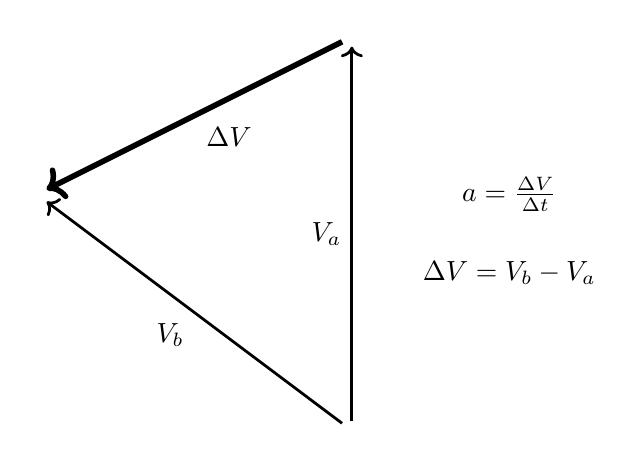
\begin{tikzpicture}[node distance=25mm]
		\node (a) at (0, 0) {};
		\node (b) at (0, 5) {};
		\node (c) at (-4, 3) {};

		\node (eqn) at (2, 3) {};
		\draw (eqn) node {$a = \frac{\Delta V}{\Delta t}$};

		\node (delv) at (2, 2) {};
		\draw (delv) node {$\Delta V = V_b - V_a$};

		\draw[->, line width=1pt] (a) to node[auto] {$V_a$} (b);
		\draw[->, line width=1pt] (a) to node[auto] {$V_b$} (c);
		\draw[->, line width=2pt] (b) to node[auto] {$\Delta V$} (c);
	\end{tikzpicture} 

	The Centripetal acceleration is due to centrepetal forces, which can be gravity or tension in a string. This can be calculated by $F = ma$. Centrepetal acceleration can also be calculated by the follwing formulas: $a = v\omega$, $a = \frac{v^2}{r}$, and $a = \omega ^2 r$. Multiplying by mass gives $F = mv\omega$, $F = \frac{mv^2}{\omega}$, and $F = m\omega^2r$

\section{Gravitation}

\subsection{Newton's Law of Gravitation}

	\begin{quote}
		Any two point masses attract each other with a force that is directly proportional to the product of their masses and inversely proportional to the square of the seperation.
	\end{quote}

	Newtons law can be summaried in the folling equations.
	
	\begin{align*}
	\text{force} &\propto \text{product  of  masses} &
		\\
		\text{force} &\propto \frac{1}{\text{distance}^2} &
		\\
		F &= \frac{GMm}{r^2} & \text{Introducing the constant G, where } G = 6.67\times 10^{-11} Nm^2kg^{-2}
	\end{align*}

\subsection{Gravitational Field Strength}

	\begin{quote}
		The gravitational field strength at a point is the gravitational force exerted per unit mass on a object at a poiny
	\end{quote}

	This is represented by $g$

	\begin{align*}g = \frac{F}{m} & & g = \frac{GM}{r^2}\end{align*}
	
\subsection{Gravitational Potential}

	\begin{quote}
		The gravitational potential at a point is the work done per unit mass to bring a abject from inifinty to a point
	\end{quote}

	It is zero at infinity and negative at any point in the universe. It is represented by the greek letter $\phi$ (phi) and is calculated using the following formula

	\[ \phi = \frac{-GM}{r} \]

\subsection{Orbiting Under Gravity}

	The equations of circular motion and gravitation can be combined to give the equation for orbits under gravity

	\[ F = \frac{mv^2}{r} = \frac{GMm}{r^2}\]
	\[ \text{so } v^2 = \frac{GM}{r}\]

	For an object in a geostationary orbit, the time period can be calculated by using the folling formula

	\[ T^2 = \left(\frac{4\pi^2}{GM}\right)r^3 \]

\section{Oscillations}

	Oscillations or vibrations are to and fro motions. They have three key properties: Frequency, amplitude and period

\subsection{Phase}

	Phase describes the point that an oscillating mass has reached within the complete cycle of an oscillation. It is often measured in degrees or radians. 

\subsection{Simple Harmonic Motion (s.h.m.)}

	There are three requirements for a mechanical system to be in s.h.m:

	\begin{itemize}
		\item
			A mass that oscillates
		\item
			A position where the mass is in equilibrium 
		\item
			A restoring force that acts to return the mass to it's equilibrium position.
	\end{itemize}

	The force is directly proportional to the displacement from the equilibrium position. The following equations describe s.h.m for a oscillator which is at the equilibrium position at $t = 0$

	\begin{align*}
		x &= x_0\sin{\omega t}
		\\
		v &= v_0\cos{\omega t}
		\\
		a &= -\omega^2x
		\\
		v &= \pm \omega \sqrt{x_0^2 - x^2}
		\\
		v_{max} &= \omega x_0
	\end{align*}

\subsection{Resonance and Damping}

	Resonance is a phenomenon observed in systems with forced oscillations. The following statements apply to systems in resonance

	\begin{itemize}
		\item
			It's natural frequency is equal to the frequency of the driver.
		\item
			It's amplitude is maximum
		\item
			It absorbs the greatest possible energy from the driver.
	\end{itemize}

	Damping is when a oscillating system loses energy (due to friction or air resistance). Critical Damping is minimum amount of energy required to return a damped system to equilibrium without oscillating

\chapter{Communication Systems}

\section{Modulation}

\subsection{F.M. and A.M.}

	When sending information over radio waves, the information must be modulated in some way. A common way of mudulating is Amplitude Modulation or AM. We can see in Fig \ref{fmamcomp} that the amplitude of the modulated wave changes to match the value of the signal. In Frequency Modulation or F.M. the frequency of the modulated wave varies with time. Example can be seen in Fig \ref{fmamcomp}

	\begin{figure}[t]
		\caption{Comparison of FM and AM \cite{taitra}}
		\label{fmamcomp}
		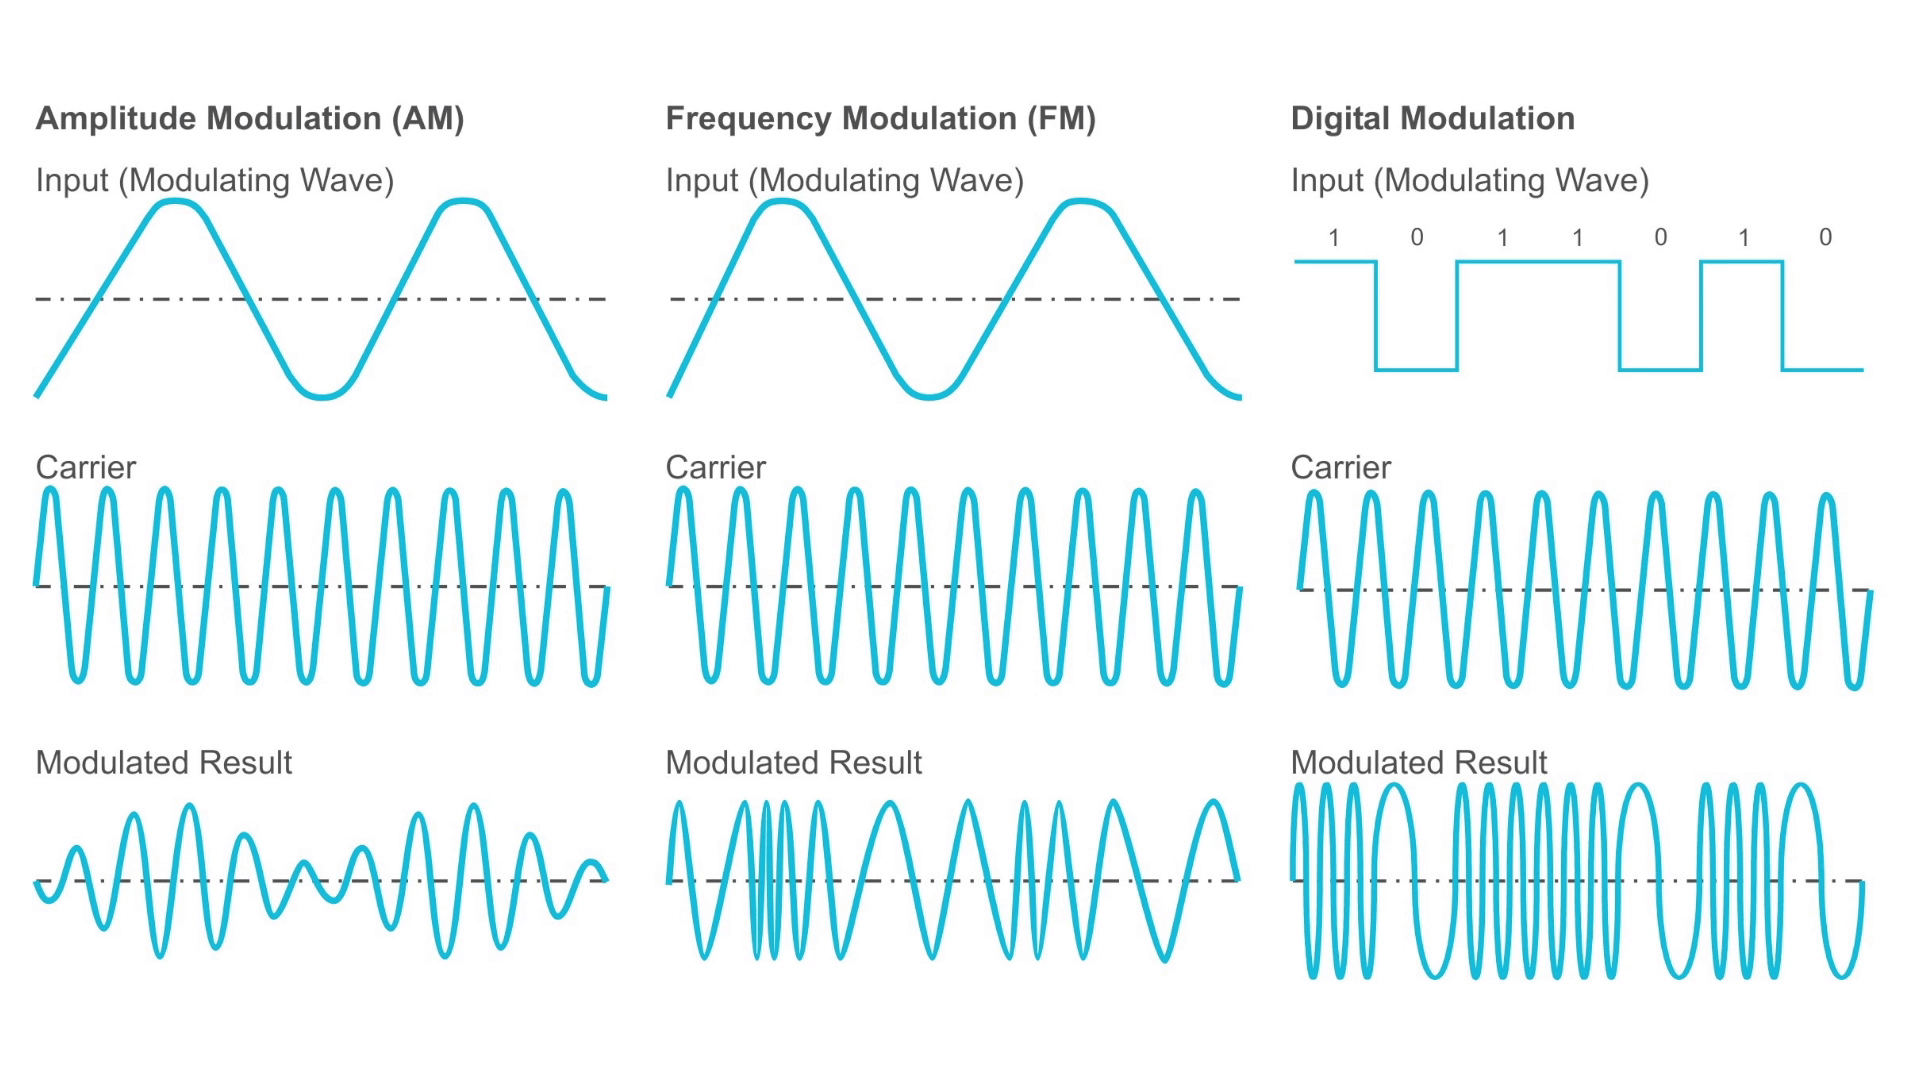
\includegraphics[width=\linewidth]{assets/fmam.png}
	\end{figure}

\subsection{Sidebands and Bandwidth}

	The frequency of the carrier wave is known as the carrier frequecny ($f_c$). When the carrier wave is modulated, it is known to carry two more frequencies called Sideband frequencies ($f_c - f_m$ and $f_c + f_m$). The bandwidth is $2f_m$

\subsection{Comparison}

	\begin{tabular}{| c | c |}
		\hline
		FM & AM \\
		\hline 
		Less Electrical Interference and Noise & Greater area covered by one transmitter \\ 
		Greater bandwidth produces better sound & Smaller bandwidth allows for more stations \\ 
		& Cheap Radio Sets \\
		\hline
	\end{tabular}

\section{Digtal Signals}

\subsection{Advantages of Digital signals}

	\begin{itemize}
		\item
			Noise can be fixed through regeneration.
		\item
			Digital Signals are more compatible with modern technologies
		\item
			Digital electronic systems are more reliable, robust and easier to build.
		\item
			Digital signals build in safegaurds so that if there is an error in recepotions, the required parts of the signal can be sent again.
	\end{itemize}

\subsection{ADC, DAC and Sampling}

	When converting between analigue and digital signals, signals must be sampled at regular intervals. The rate at which it is sampled is called the Sample Rate. The resoultion at which the signal is sampled is called the bit-depth


\section{Crosstalk and Signal Attenuation}

	\begin{quote}
		Crosstalk or Crosslinking occurs when a signal transmitter in one circuit or channel creates an undesired effect in another circuit or channel
	\end{quote}

	\begin{quote}
		Signal Attenuation is the gradual decrease in power of a signal the further it travels.
	\end{quote}

	The decrease in power from $P_1$ to $P_2$ can be very high. A $\log_{10}$ is used and the ratio is reprented in Bels (often multiplied by 10 and written as deciBels or dB)

	\[ \text{Attenuation}  = 10\log_{10}\left(\frac{P_1}{P_2}  \right) \text{dB}\]

\section{Channels of Communications}

\subsection{Wire Pairs and Co-axial cables}

	Telephones used to use pairs of wires to carry signals. The difference in the Potential differences of the wires was the signal, but they easily picked up noise. The closer the wires were, the less noise was picked up, so they were twisted together.

	Coaxial reduces the amount of crosstalk in the wire when the transmission occurs at high speeds. The copper core usually carries the signal and the copper braid (mettalic shield) is connected to earth. see Fig \ref{coaxial} Since electromagnetic radiation does not travel easily through metal, inteference does not occur at the core.

	\begin{figure}[t]
		\label{coaxial}
		\caption{A Coxial Cable \cite{wikicomm:coax}}
		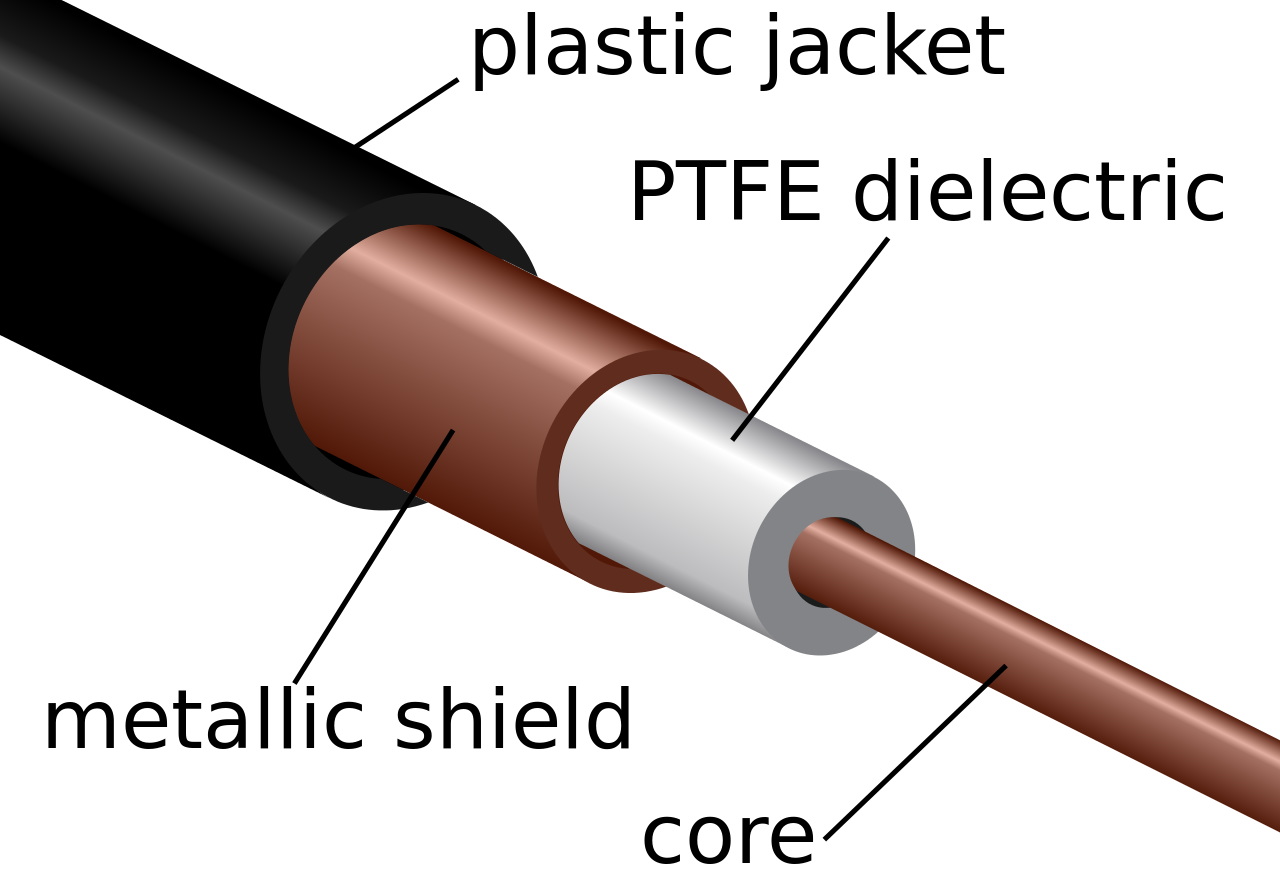
\includegraphics[width=\linewidth]{assets/coaxial.png}
	\end{figure}

	\begin{tabular}{| c | c |}
		\hline
		Wire Pairs & Coaxial \\
		\hline 
		Cheap and convenient & Expensice \\
		Strongly attenuate signal & Less attenuating \\ 
		Low bandwidth & High bandwidth \\ 
		Pushes up inteference/noise & Less inteference and noise \\ 
		Crosstalk & less Crosstalk \\ 
		Low security & More secure \\ 
		\hline
	\end{tabular}

\subsection{Radio Waves and Microwave links}

	Various electromagnetic waves are used to carry informations. In waves such as skywaves, the ionosphere is used to reflect the waves.

	\begin{tabular}{| c | c | c |}
		\hline
		Type & Frequency Range & Distance Travelled \\
		\hline
		Surface wave & upto 3MHz & upto 1000Km \\
		Sky wave & 3 - 30MHz & Worldwide by reflection \\
		Space wave & 30 - 300MHz & line of sight \\
		Microwave & 1-300GHz & line of sight, except when retransmitted by sattelite \\
		\hline
	\end{tabular}

\subsection{Sattelites and Optic fibre}

	Sattelites offer some extra advantages over skywaves

	\begin{itemize}
		\item
			The concentration of ions in the ionosphere is constantly changing and the reflection of skywaves is not always possible
		\item
			The sattelite boosts the signal for its return to earth.
		\item
			Sattelite communications use higher frequencies and hence have height bandwidth
		\item
			More channels are available for communicating on higher frequencies
	\end{itemize}

\chapter{Thermal Physics}

\section{Changes of state}

\subsection{Energy Changes}

       When a solid is heated, it's temperature starts rising and it's molecules gain kinetic energy. When the solid reaches it's melting point, the heat energy is used to break the intermolacular bonds. The temperature remains constant but the seperation between the particles significantly increases and hence the potential energy of the molecules increases. The solid starts melting. After the solid has completally melted, the temperature starts rising again and the Kinetic energy increases until the liquid reaches it's boiling point. Again, the heat energy is used up in breaking up intermolecular bonds, and the temparature stops rising untill all of the liquid has turned into gas. After that the temperature continues to increase velocity. A summary can be seen in Fig. \ref{energych}

       \begin{figure}[h]
	       \caption{Energy Changes \cite{edplace:ech}}
               \label{energych}
               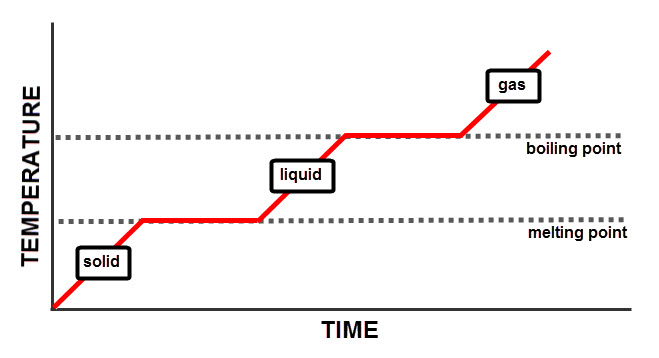
\includegraphics[width=\linewidth]{assets/EnergyChanges.jpg}
       \end{figure}

       The energy supplied to a substance when it is channging state (at a constant temperature) is called the latent heat of change in state for that material.

\subsection{Evaporation}

	Liquids can change into gasses without reaching boiling point. In a liquid some molecules move faster than the others. These molecules break free and form a vapor above the liquid. This is called evaporation. Since higher energy particles leave the liquid, the temperature of the liquid decreases.

\section{Internal Energy}

\subsection{Energy of the particles}

	\begin{quote}
		The internal energy of a system is the sum of the random distribution of kinetic and potential energies of it's atoms or molecules
	\end{quote}

	There are two ways in which the internal energy of a system can be increased.

	\begin{itemize}
		\item
			\textbf{By heating the system} : When a material is heated, the kinetic energy of the particles increases.
		\item
			\textbf{By doing work on the system} : When a gas is compressed, the molecues strike the walls and move faster.
	\end{itemize}

\subsection{What is Temperature}

	Temperature is a measure of the average kinetic energy of the particles in the system. A common scale is the celsius scale, where \SI{0}{\celsius} is the freezing point of water and \SI{100}{\celsius} is the boiling point of water. The Termodynamic or Kelvin scale uses the absolute zero as \SI{0}{\kelvin}. For matter at absolute zero, it is impossible to remove any more energy out of it. The other fixed point is at \SI{273.15}{\kelvin}, the triple point of water.

	\[ \theta (\SI{}{\celsius}) = T (\SI{}{\kelvin}) -273.15 \]

\subsection{The First Law of Thermodynamics}

	\begin{quote}
		The first law of thermodynamics states that the total energy of an isolated system remains constant.
	\end{quote}

	This means that the energy supplied to a system by heating it or doing work on it increases the internal energy of the system.

	\begin{align*}
		\text{Increase in internal energy} &= \text{Energy supplied by heating} +  \text{Energy supplied by doing work} \\
		\Delta u &= q + w
	\end{align*}

\section{Thermometers}

\subsection{Types of thermometers}

	Thermometers are devices that are used to measure temperature. They use some property of the material which changes with temperatures. This could be:

	\begin{itemize}
		\item
			The resistance of a electrical resistor
		\item
			The voltage produced by a thermocouple
		\item
			The color of an electrically heated wire
		\item
			The volume of a fixed mass of gas at constant pressure
	\end{itemize}

\subsection{Thermocouple thermometer vs. Resistance thermometer}


	\begin{tabular}{| p{0.2\linewidth} | p{0.4\linewidth} | p{0.4\linewidth} |}
		\hline
		Feature & Resistance thermometer & Thermocouple thermometer \\
		\hline
		robustness & very robust & robust \\
		range & Thermistor: narrow range, resistance wire: wide range & can be wide \\
		size & larger than thermocouple, has greater thermal capacity therefore slower acting & smaller than resistance thermometers, has smaller thermal capacity, so quicker acting and can measure temperature at a point \\
		sensitivity & Thermistor: high sensitivity over narrow range, resistance wires: less sensitive & can be sensitive if appropriate metal are chosen \\
		linearity & Thermistor : fairly linear over narrow range, resistance wire: good linearity & non-linear so requires callibiration \\
		remote operation & long conducting wires allow the operator to be at a distance from the thermometer & long conducting wires allow the operator to be at a distance from the termometer \\
		\hline
	\end{tabular}

\section{Calculating energy changes}

\subsection{Specific heat capacity}

	\begin{quote}
		The specific heat capacity of a substance is the energy required per unit mass of the substance to raise the temperature by \SI{1}{\kelvin}
	\end{quote}

	This can be represented with the following formula

	\begin{align*}
		\text{Specific heat capacity} &= \frac{\text{energy supplied}}{\text{mass} \times \text{temperature change}} \\
		C &= \frac{E}{m\Delta\theta}
	\end{align*}

\subsection{Specific latent heat}

	\begin{quote}
		The specific latent heat of a substance is the energy per kilogram of the substance to change it's state without any change in temperature
	\end{quote}

	When a substance melts, the quantity is called the specific latent heat if fusion; for boiling, it's the specific latent heat of vaporisation.

	\[ \text{latent heat} = \frac{\text{Energy to change state}}{\text{mass}} \]

\chapter{Electromagnetism}

\section{Electric Fields}

\subsection{Coulomb's Law}

	An electrically charged object produces an electric field on the space around it. This field exerts a force on the other charged objects in the field. Coulomb's law describes this force.

	\begin{quote}
		Any two point charges exert an electrical force on each other that is proportional to the product of the charges and inversly proportional to the square of the distance between them.
	\end{quote}

	This law can be mathematically represented as,

	\begin{align*}
		F \propto \frac{1}{r^2} &&
		F \propto Q_1 Q_2
	\end{align*}

	Combining and resolving the proportionality results in, 

	\begin{align} 
		F = \frac{Q_1 Q_2}{4\pi \epsilon_0 r^2 } \label{coulombslaw}
	\end{align}

	Here $\frac{1}{4\pi \epsilon_0}$ is the constant of proportionality, and $\epsilon_0$ is called the permitivity of free space. It equals approximatally \SI{8.85}{\farad\per\meter}

\subsection{Electric field strength}

	\begin{quote}
		The electric field strength at a point is the force per unit charge exerted on a stationary positive charge at that point
	\end{quote}

	Mathematically, 

	\begin{align}
		F = \frac{E}{Q} \label{elecfstr}
	\end{align}

	For a uniform electric field between charged parallel plates, it is also,

	\[ E = \frac{V}{d} \]

	Where, V is the potential difference between the plates, and d is the distance between them.

	To calculate the electric field strength for a radial field we can combine the formulas \ref{coulombslaw} and \ref{elecfstr},

	\begin{align*}
		& E = \frac{Q_1 Q_2}{4\pi \epsilon_0 r^2 Q_2} \\
		\implies &  E = \frac{Q}{4\pi \epsilon_0 r^2}
	\end{align*}

\section{Electric potential}

\subsection{Energy changes in a uniform field}

	Electrical potential energy is the potential energy of a charge due to itsposition in a electric field. The electric potential at a point is the potential energy per unit charge at that point.

	In a uniform field, this can be represented as,

	\begin{align}
		V = \frac{W}{Q} \label{unielecpot}
	\end{align}
	
	Where, V is the electric potential, Q is the charge, and W is the work done in maving the charge from the negative plate to the positive plate. The potential of zero is defined as "earth" or "ground".

\subsection{Energy changes in a radial field}

	The electric field strength increases as we move closer to a charged object. To calculate the electric potentialwe can integrate the equation for coulomb's law, equation \ref{coulombslaw}, and combine it with equation \ref{unielecpot} to get.

	\[ V = \frac{Q}{4\pi \epsilon_0 r} \]

	Here the zero potential is defined as the potential at a infinite distance away from the charge.

\subsection{Defining electric potential}

	\begin{quote}
		The electric potential at a point is equal to the work done in bringing unit positive charge from infinity to a point
	\end{quote}

\section{Comparing gravitational and electric forces}

	\begin{tabular}{| p{0.5\linewidth} | p{0.5\linewidth} |}
		\hline
		Gravitational Field & Electric fields \\
		\hline \hline
		\textbf{Origin: } \newline Arises from masses & \textbf{Origin: } \newline Arise from electric charges \\ \hline
		\textbf{Vector forces: } \newline Only gravitational attraction, no repulsion & \textbf{Vector forces: } \newline Both electrical attraction and repulsion are possible (because of positive and negative charges) \\ \hline
		\textbf{All gravitional fields: } \newline field strength \newline $g = \frac{F}{m}$. \newline i.e. field strength is force per unit mass & \textbf{All electric fields: } \newline field strength \newline $E = \frac{F}{Q}$. \newline i.e. field strength is force per unit positive charge \\ \hline
		\textbf{Units: } \newline $F$ is in \SI{}{\newton}, $g$ is in \SI{}{\newton\per\kilo\gram} or \SI{}{\meter\per\second} & \textbf{Units: } \newline $F$ is in \SI{}{\newton}, $E$ is in \SI{}{\newton\per\coulomb} or \SI{}{\volt\per\meter} \\ \hline
		\textbf{Uniform gravitational fields: } \newline parallel gravitational field lines \newline $g = \text{constant}$ & \textbf{Uniform electric fields: } \newline parallel electric field lines \newline $E = \frac{V}{d} = \text{constant}$ \\ \hline
		\textbf{Spherical gravitional fields: } \newline radial field lines \newline force given by Newton's laws: $F = \frac{GMm}{r^2}$ \newline field strength is therefore: $g = \frac{GM}{r^2}$ \newline (force and field strength obey an inverse square law with distance) & \textbf{Spherical electric fields: } \newline radial field lines \newline force given by coulomb's law: $F = \frac{Q_1 Q_2}{4\pi \epsilon_0 r^2}$ \newline field strength is therefore: $E = \frac{Q}{4\pi \epsilon_0 r^2}$ \newline force and field strength obey an inverse square law with distance \\ \hline
		\textbf{Gravitational potential: } \newline given by $\phi = -\frac{GM}{r}$ \newline potential obeys an inverse relationship with distance and is zero at ininity \newline potential is a scalar quantity and is always negative & \textbf{Electic potential: } \newline given by: $V = \frac{Q}{4\pi \epsilon_0 r}$ \newline potential obeys an inverse relationship with distance and is zero at infinity \newline potential is scalar quantity \\ \hline
	\end{tabular}

\section{Capacitors}

\subsection{What are Capacitors}

	\begin{wrapfigure}{R}{0.4\linewidth}
		\centering
		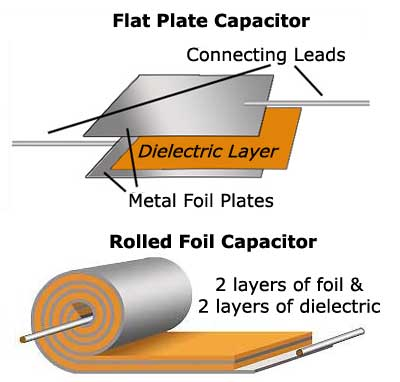
\includegraphics[width=\linewidth]{assets/capacitor.jpg}
		\caption{Construction of a Capacitor. \cite{lrnabtelec:cap}}
		\label{capint}
	\end{wrapfigure}

	Capacitors are elecronic devices that store energy, and gradually release it. They have two leads connected to two plates seperated by an insulating material called the \textbf{dielectric} When a potential difference is applied across the terminals of a capacitor, equal and opposite charges are stored on the plates. When the potential difference is removed, the stored charge produces it's own volatge. if the capacitor is connected to a complete circuit, then the charge flows out releasing the energy. Figure \ref{capint} shows the construction of a capacitor.

\subsection{Capacitance}

	Different Capacitors have different capacities to store charge. Capacitance is a measure of how much charge a capacitor can store. The greater the capacitance, the greater charge a capacitor stores for a given potential difference acroes it.

	\begin{quote}
		The capacitance of a capacitor is the charge stored on one plate per unit potential difference between the plates.
	\end{quote}

	Mathematically,

	\begin{align}
		\text{Capacitance} &= \frac{\text{Charge}}{\text{Potential difference}} \notag \\
		C &= \frac{Q}{V} \label{capacitanceeq}
	\end{align}

	The unit of capacitance is the \textbf{farad}, \SI{}{\farad}

	\[ \SI{1}{\farad} = \SI{1}{\coulomb\per\volt} \]

\subsection{Energy stored in a capacitor}

	\begin{wrapfigure}{R}{0.4\linewidth}
	\caption{Potential Difference against charge}
	\centering
	\label{pdvcap}
	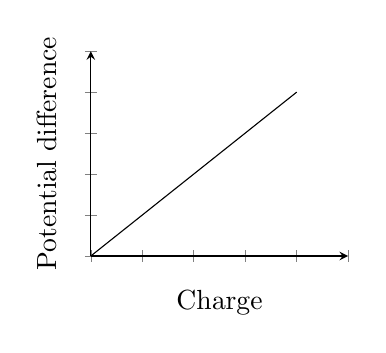
\begin{tikzpicture}
		\begin{axis}[
			xlabel={Charge},
			ylabel={Potential difference},
			xticklabels={,,},
			yticklabels={,,},
			xmin=0,
			xmax=10,
			ymin=0,
			ymax=10,
			domain=0:8,
			axis x line=bottom,
			axis y line=left,
			width=0.4\textwidth
			]
			\addplot[no marks]{x};
		\end{axis}
	\end{tikzpicture}
	\end{wrapfigure}
	
	As the charge stored in a capacitor increases, the repulsion makes it harder to store more charge in the capacitor, and more energy us required. Fig \ref{pdvcap} shows a graph of Voltage against charge on a capacitor. The work done in moving charge $Q$ across a potential difference of $V$ is the product $QV$. Here, the work done is the area under the graph of figure \ref{pdvcap}, 

	\begin{align}
		W = \frac{1}{2}QV \label{capawork}
	\end{align}

	by substituting equation \ref{capacitanceeq} into equation \ref{capawork} we get two new equations,

	\begin{align}
		W &= \frac{CV^2}{2} \\
		W &= \frac{Q^2}{2C}
	\end{align}

\section{Capacitors in a circuit}

\subsection{Capacitors in parallel}

	When two capacitors are connected in parallel, they are equivalent to a single capacitor with larger plates. Hence their combined capacitance is the sub of their individual capacitances.

	\[ C_{\text{total}} = C_1 + C_2 + C_3 + \text{...} \]

	\begin{figure}[h]
	\caption{Capacitors in parallel}
	\label{capinpar}
	\centering
	\begin{circuitikz} \draw
		(0, 0) -- (1, 0)
		(1, 0) -- (1, 1)
		to[capacitor, C=$C_1$] (5, 1)  -- (5, 0)
		(1, 0) -- (1, -1)
		to[capacitor, C=$C_2$] (5, -1) -- (5, 0)
		-- (6, 0)
		;
	\end{circuitikz}
	\end{figure}

\subsection{Capacitors in series}

	For a system where capacitors are connected in series, like in fig \ref{capinser}, the reciprocal of the cotal capacitance is the sub of the reciprocal of the individual capacitances.

	\[ C_{\text{total}} = \frac{1}{C_1} + \frac{1}{C_2} + \frac{1}{C_2} + \text{...} \]

	\begin{figure}[h]
	\caption{Capacitors in series}
	\label{capinser}
	\centering
	\begin{circuitikz}
		\draw
		(0, 0) to[capacitor, C=$C_1$] (2, 0) to[capacitor, C=$C_2$] (4, 0)
		;
	\end{circuitikz}
	\end{figure}

\subsection{Sharing charge between capacitors}

	\begin{wrapfigure}{R}{0.3\linewidth}
	\caption{Capacitors charing charges}
	\label{capshare}
	\centering
	\begin{circuitikz} \draw
		(0, 0) -- (0, 1) to[capacitor, C=$C_1$] (2, 1) 
		(0, 0) -- (0, -1) to[capacitor, C=$C_2$] (2, -1) -- (2, 1)
		;
	\end{circuitikz}
	\end{wrapfigure}

	If a capacitor, with a capacitance of $C_1$ is charged with a power supply to a voltage of $V_{\text{init}}$, and then connected to a second capacitor with capacitance $C_2$, the charge is shared between the capacitors. As showen in Figure \ref{capshare}, the capacitors are in parrallel, so the capacitance is calculated by, 
	\begin{align*}
		C_{\text{total}} &= C_1 + C_2 \\
		Q &= C_1 V_{\text{init}}
	\end{align*}

	Since charge is conserved, we can calculate the potential difference across the capacitors as,

	\[ V_{\text{new}} = \frac{Q}{C_{\text{total}}} \]

\section{Capacitance of isolated bodies}

	All bodies have capacitance. For a conducting sphere of radius $r$ insuated from its surroundings, carring a charge of $Q$, will have a potentail on the surface of $V$, and a capacitance of $C$, where,

	\begin{align*}
		V = \frac{Q}{4\pi\epsilon_0 r} && C = 4\pi\epsilon_0 r
	\end{align*}

\printbibliography{}
\end{document}
